\documentclass[11pt,a4paper,titlepage,brazil]{article}
\usepackage[brazilian]{babel}
\usepackage[T1]{fontenc}
\usepackage[utf8]{inputenc}
\usepackage[a4paper]{geometry}
\geometry{top=2.0cm, bottom=2.0cm, left=2.0cm, right=2.0cm}
\usepackage{setspace}
\usepackage{libertine}
\usepackage{graphicx}

\begin{document}

\begin{center}
 \large{\textbf{Descrição: Natalí Soler Matubaro de Santi}}\\
\end{center}

Sou física teórica e meus principais interesses se concentram em aprendizado de máquina, ciência de dados, cosmologia, física computational, relatividade geral e teoria quântica de campos. Sou bacharela em física pela Universidade de São Paulo (USP), campus de São Carlos em 2015 e mestra em física pela Universidade Federal de São Carlos (UFSCar), campus de São Carlos, em 2018. Atualmente realizo meu doutorado em Cosmologia pela Universidade de São Paulo (USP), campus de São Paulo. Possuo experiência em física de partículas, produção e caracterização de materiais, teoria quântica de campos, teoria quântica de campos em espaços curvos e termodinâmica de buracos negros.

\begin{figure}[h!]
 \centering
 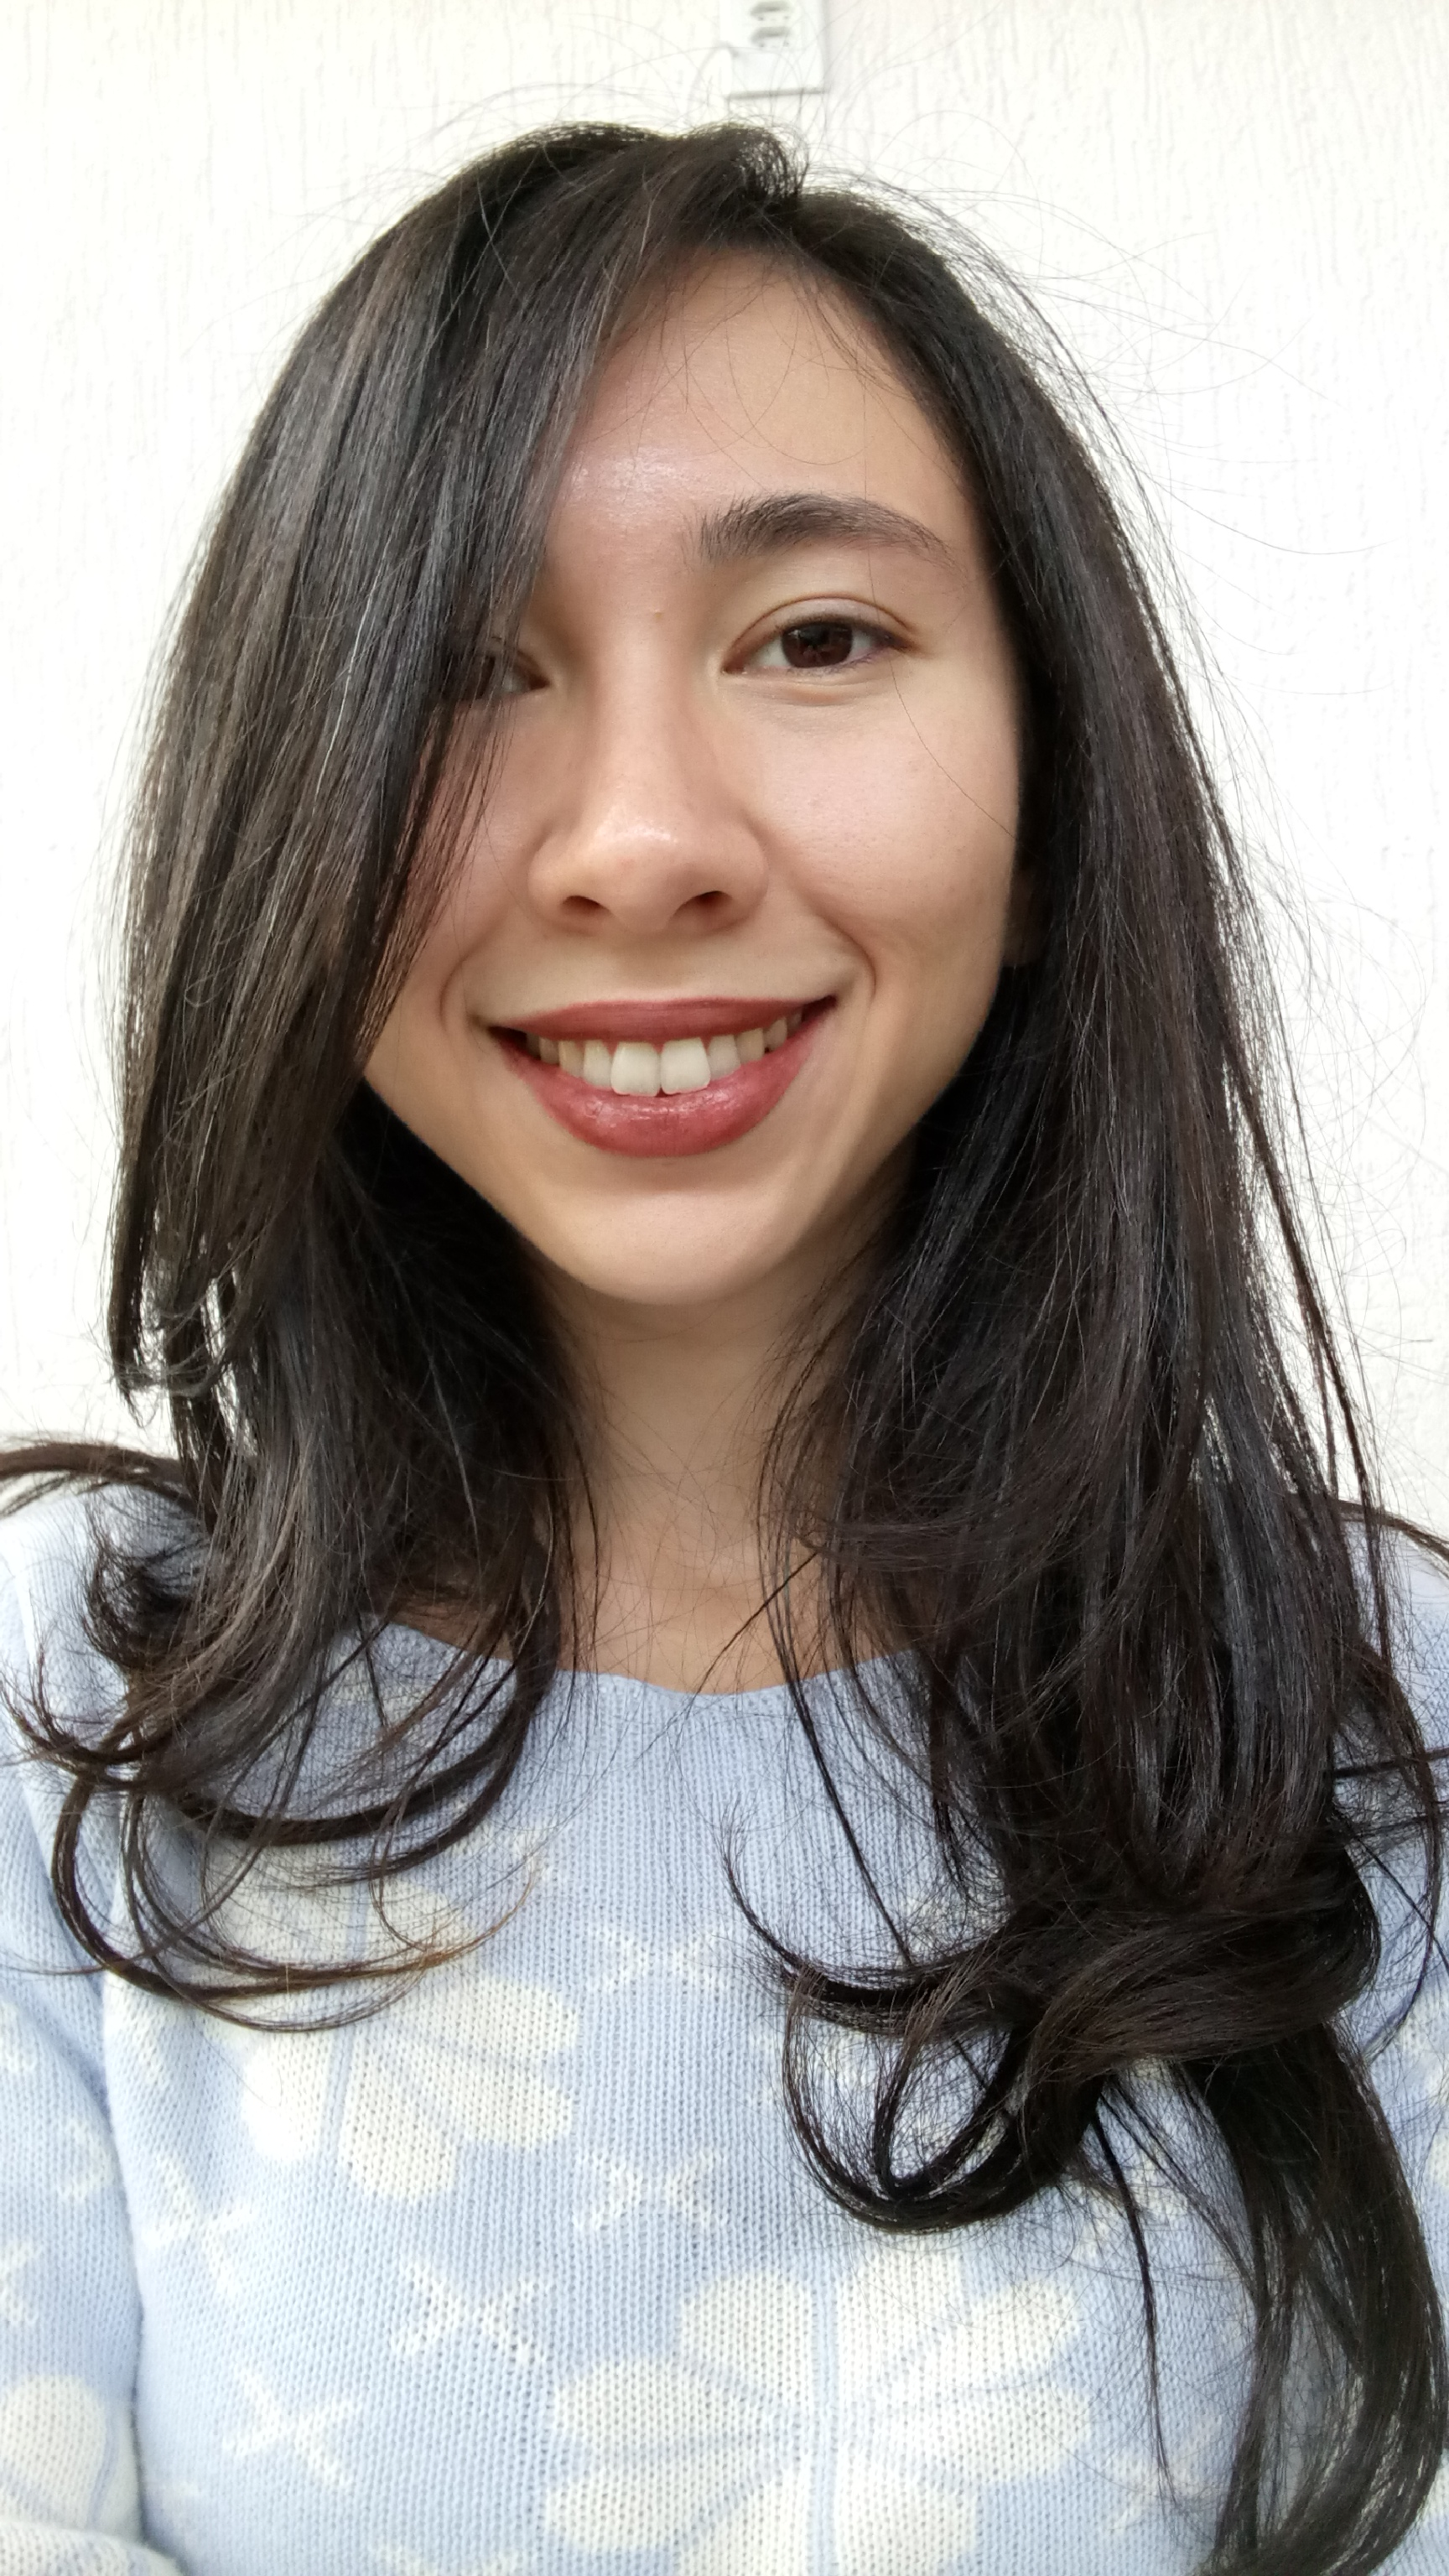
\includegraphics[scale=0.1]{natalidesanti.jpg}
\end{figure}  

\end{document}

%%% Local Variables:
%%% mode: latex
%%% TeX-master: t
%%% End:
